\subsection{Disk Storage and Files}


\subsubsection{Physical Storage Media}

The storage media can be organized into a \textbf{storage hierarchy}.
\begin{itemize}[label=\(\rhd\)]
    \item \textbf{Classification} of storage media:
    \begin{itemize}[label=\(\rhd\)]
        \item \textbf{Speed} with which data can be accessed
        \item \textbf{Cost} per unit of data
        \item \textbf{Reliability}
        \begin{itemize}[label=\(\rhd\)]
            \item data loss on power failure or system crash
            \item physical failure of the storage device
        \end{itemize}
        \item \textbf{Volatile} vs. \textbf{non-volatile} storage
        \begin{itemize}[label=\(\rhd\)]
            \item Volatile (non-volatile): losses (persists) content when power is switched off
        \end{itemize}
    \end{itemize}
    \item \textbf{Primary storage}: Fastest media, but volatile
        \begin{itemize}[label=\(\rhd\)]
            \item \textbf{Cache} $\approx 3$ clock cycles fbox{$\eta$-sec}
            \begin{itemize}[label=\(\rhd\)]
                \item Fastest and most costly form of storage
                \item Managed by the computer system hardware
            \end{itemize}
            \item \textbf{Main memory} $\approx 100 clock cycles$ \fbox{$\eta$-sec}
            \begin{itemize}[label=\(\rhd\)]
                \item Fast access
                \item Generally only part of a database is loaded into memory
            \end{itemize}
        \end{itemize}
    \item \textbf{Secondary storage}: Non-volatile, moderately fast access
    \begin{itemize}[label=\(\rhd\)]
        \item \textbf{Flash memory (SSD)} \fbox{$\mu$-sec}
        \begin{itemize}[label=\(\rhd\)]
            \item Reads are roughly as fast as main memory
            \item Writes are slow 
        \end{itemize}
        \item \textbf{Magnetic disk} \fbox{$m$-sec}
        \begin{itemize}[label=\(\rhd\)]
            \item Data is stored on spinning disk, and read/written magnetically
            \item Much slower access than main memory; much larger capacity
            \item Data must be moved from disk to main memory for access and written back for storage
            \item Direct data access, i.e., data can be read in any order
        \end{itemize}
    \end{itemize}
    \item \textbf{Tertiary storage}: Non-volatile, slow access time
    \begin{itemize}[label=\(\rhd\)]   
        \item \textbf{Optical disk} \fbox{m-sec /sec}
        \begin{itemize}[label=\(\rhd\)]
            \item Data is read optically from a spinning disk using a laser
            \item Slower than magnetic disk
        \end{itemize}
        \item \textbf{Tape storage} \fbox{sec/min/hours}
        \begin{itemize}[label=\(\rhd\)]
            \item Much slower
            \item Sequential access only
            \item Very high capacity
            \item Tape storage costs much cheaper than disk storage costs
        \end{itemize}
    \end{itemize}
\end{itemize}

\textbf{Performance measures} of hard disks:
\begin{itemize}[label=\(\rhd\)]
    \item \textbf{Access time}: the time it takes from when a read or write request is issued to when the data transfer begins. Is composed of:
    \begin{itemize}[label=\(\rhd\)]
        \item \textbf{Seek time}: time it takes to reposition the arm over the correct track 
        \item \textbf{Rotational latency}: time it takes for the sector to be accessed to appear under the head
    \end{itemize}
    \item \textbf{Data-transfer rate}: rate at which data can be retrieved from or stored to disk
    \item \textbf{Mean time to failure (MTTF)}: avg. time the disk is expected to run continuously without failure
\end{itemize}

\subsubsection{Accessing the Storage}
\begin{itemize}[label=\(\rhd\)]
    \item A \textbf{block} is a contiguous sequence of sectors from a single track
    \item Blocks are separated by \textbf{interblock gaps}, which hold control information created during disk initialization
    \item Logically, a block is a unit of storage allocation and data transfer
\end{itemize}

\rule{\linewidth}{0.4pt}

\textbf{\underline{Example Calculation}}\\
Consider relations $r(A)$ and $s(A)$. $r$ is ordered, $s$ is unordered. Block size $B=2KB$. Tuple size $t=100$Bytes. $|r|=|s|=800'000$ tuples. The values of A are uniformly distributed between 5M and 10M. The time for 1 IO is 0.025 sec. Determine the execution times for the following queries where $x=r$ or $x=s: \sigma_{A=6M}(x), \sigma_{A<5'000'500}(x), \sigma_{A\neq 6M}(x)$.
\begin{align*}
    &- \frac{2M}{100} = 20 \text{ tuples per block} \\
    &- \frac{800'000}{20} = 40'000 \text{ blocks}
\end{align*}

\rule{250pt}{0.4pt}
\begin{align*}
    \sigma_{A = 6M}(r) : &\text{ binary search on contiguous blocks} \\
    &\log_2 40'000 \cdot 0.025 \text{ sec} = 0.38 \text{ sec}
\end{align*}

\begin{align*}
    \sigma_{A = M}(s) : &\text{ scan half of S on avg. if A is unique} \\
    &20'000 \cdot 0.025 \text{ sec} = 500 \text{ sec}
\end{align*}

\begin{align*}
    \sigma_{A \leq 5000'500}(r) \\
    &\bullet \text{ avg. distance between values} = \frac{5M}{800'000} = 6.25 \\
    &\bullet \text{ nr. of qualifying tuples} = \frac{500}{6.25} = 80 \text{ tuples} \\
    &\bullet \text{ nr. of qualifying blocks} = \left\lceil \frac{80}{20} \right\rceil = 4 \text{ blocks} \\
    &0.025 \cdot 4 = 0.1 \text{ sec}
\end{align*}

\begin{align*}
    \sigma_{A<5'000'500}(s): &0.025\cdot 40'000= 1000 \text{ sec}\\
    \sigma_{A\neq 5M}(s): &\text{ scan the relation} \\
    &0.025 \cdot 40'000 = 1000 \text{ sec}
\end{align*}
\rule{\linewidth}{0.4pt}

Techniques to optimize disk-block access:
\begin{enumerate}
    \item Disk arm scheduling
    \item Appropriate file organization
    \item Write buffers and log disks
\end{enumerate}

\subsubsection{Buffer Manager}
\begin{itemize}[label=\(\rhd\)]
    \item \textbf{Buffer}: Portion of main memory available to store copies of disk blocks
    \item \textbf{Buffer Manager}: Subsystem that is responsible for buffering disk blocks in main memory
\end{itemize}

\subsubsection{Organization of Files}
\begin{itemize}[label=\(\rhd\)]
    \item \textbf{File}: A file is logically a \textbf{sequence of records}, where
\end{itemize}

\subsection{Index Structures}

\subsubsection{Basic Concepts}
\begin{itemize}[label=\(\rhd\)]
    \item \textbf{Index file:} Consists of records (called \textbf{index entries}) of the form (\textit{search key, pointer}) where
    \begin{itemize}[label=\(\rhd\)]
        \item \textbf{search key} is an attribute or set of attrs. used to look up records in a data file
        \item \textbf{pointer} is a pointer to a record (database tuple) in a data file
    \end{itemize}
    \textbf{Evaluation of an index} must include:
    \begin{itemize}[label=\(\rhd\)]
        \item Access time, insertion time, deletion time, space overhead
    \end{itemize}
    \item Depending on the ordering of the data and the index file we can have a 
    \begin{itemize}[label=\(\rhd\)]
        \item \textbf{clustering index} (same order of data and index)
        \item \textbf{non-clustering index} (different order of data and index)
    \end{itemize}
    \item Depending on what we put into the index we have a 
    \begin{itemize}[label=\(\rhd\)]
        \item \textbf{sparse index} (index entry for some tuples only)
        \item \textbf{dense index} (index entry for each tuple)
    \end{itemize}
    \item A clustering index is usually sparse
    \item A non-clustering index must be dense
\end{itemize}

\subsubsection{Clustering Index}
\begin{itemize}[label=\(\rhd\)]
    \item In a clustering index the search key order corresponds to the sequential order of the records in the data file
\end{itemize}
\subsubsection{Non-Clustering Index (Secondary Indexes)}
\begin{itemize}[label=\(\rhd\)]
    \item Non-clustering index: index whose search key specifies an order different from the sequential order of the file
    \item Must be dense
    \item Two options for data pointers:
    \begin{itemize}[label=\(\rhd\)]
        \item Duplicate index entries: an index records for every data record
        \item Buckets: An index records for each search key value; index record points to a \textbf{bucket} that contains pointer to all the actual records with that particular search key value
    \end{itemize}
\end{itemize}

\subsubsection{Mutlilevel Index}
\begin{itemize}[label=\(\rhd\)]
    \item Inner index: The main index file for the data
    \item Outer index: A sparse index on the index
\end{itemize}


\subsubsection{B+ Tree}
\begin{itemize}[label=\(\rhd\)]
    \item The \textbf{B+ tree} is a mutli-level index and is the alternative to sequential index files  
    \item B+ Tree: a rooted tree with the following properties
\begin{figure}[H]
    \centering
    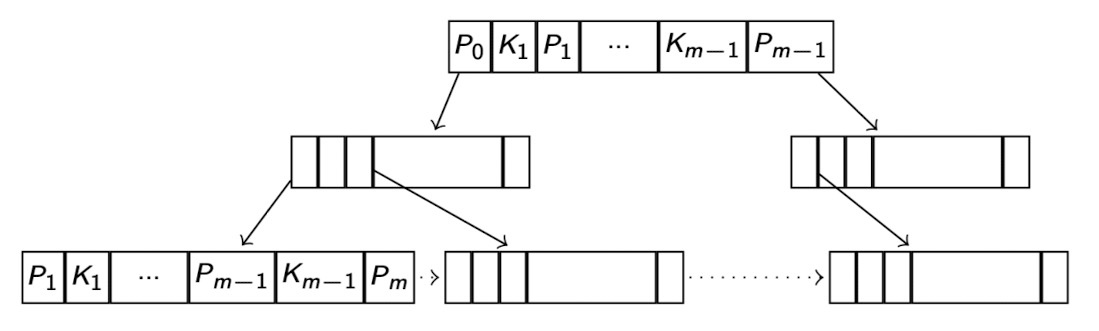
\includegraphics[width=0.75\linewidth]{Screenshot 2024-05-22 at 15.43.01.jpg}
\end{figure}
\begin{itemize}[label=\(\rhd\)]
    \item \textbf{Balanced tree}, i.e. all paths from root to leaf are of the same length (at most $\lceil \log_{\lceil m/2\rceil}(K)\rceil$ for K search key values)
    \item A \textbf{node} contains up to $m-1$ search key values and $m$ pointers, and the search key values within a node are sorted
    \item Nodes are between half and completely full
    \item \textbf{Internal nodes} have between $\lceil m/2 \rceil$ and $m$ children (= between $\lceil m/2\rceil -1 $ and $m-1$ search key values)
    \item \textbf{Leaf nodes} have between $\lceil (m-1)/2 \rceil$ and $m-1$ search key values
    \item \textbf{Root node}: If it is a leaf, it can have between 0 and $m-1$ search key values, otherwise it has at least 2 children
\end{itemize}
\item Observations about B+ Trees:
\begin{itemize}[label=\(\rhd\)]
    \item Search is efficient, since only a small number of index blocks need to be read
    \item Insertions and deletions to the main file can be handled efficiently, as the index can be restructured in logarithmic time
\end{itemize}
\item Queries on B+ trees:
\begin{itemize}[label=\(\rhd\)]
    \item Steps to find all records with a search key value of $k$ (assume dense index)
    \begin{enumerate}
        \item Set $C=$ root node
        \item \textbf{while} C is not a leaf node \textbf{do}
        \begin{itemize}[label=\(\rhd\)]
            \item[] Search for the largest search key value $\leq$ k
            \begin{itemize}[label=\(\rhd\)]
                \item[] \textbf{if} such a value exists, assume it is $K_i$
                \item[] \textbf{then} set $C=$ the node pointed to by $P_i$
                \item [] \textbf{else} set $C= $ the node pointed to by $P_0$
            \end{itemize}
        \end{itemize}
        \item If there is a key value $K_i$ in $C$ such that $K_i=k$
        \begin{itemize}[label=\(\rhd\)]
            \item[] \textbf{then} follow pointer $P_i$ to the desired record or bucket
            \item[] \textbf{else} no record with search key value $k$ exists
        \end{itemize}
    \end{enumerate}
\end{itemize}
    \item B+ Tree Insertions - Intuition
    \begin{itemize}[label=\(\rhd\)]
    \item Insert a record with search key value of $k$
    \begin{enumerate}[left=0pt, itemsep=1ex, label=\textcolor{black}{\arabic*.}, font=\bfseries]
        \item Find the leaf node in which the search key value would appear
        \item If the search key value is already there \textbf{then}
        \begin{itemize}[label=\(\rhd\)]
            \item[] Add record to the data file
        \end{itemize}
        \item If the search key value is not there and leaf is not full \textbf{then}
        \begin{itemize}[label=\(\rhd\)]
            \item[] Add record to the data file
            \item[] Insert (pointer, key-value) pair in the leaf node such that the search keys are still in order
        \end{itemize}
        \item If search value is not there and leaf is full \textbf{then}
        \begin{enumerate}[left=1em, itemsep=1ex, label=\textcolor{black}{\arabic{enumi}.\arabic*.}]
            \item Take all entries (including the new one being inserted) in sorted order; place the first half in the original node and the rest in a new node
            \item Insert the smallest entry of the new node into the parent of the node being split
            \item If the parent is full \textbf{then} split it and propagate the split further up
        \end{enumerate}
    \end{enumerate}
    \item Splitting propagates upwards until a not full node is found
    \begin{itemize}[label=\(\rhd\)]
        \item In the worst case the root is split, increasing the tree height by 1
    \end{itemize}
\end{itemize}
    \item B+ Tree Deletions - Intuition
    \begin{itemize}[label=\(\rhd\)]
        \item Deletion of a record with search key $k$
        \begin{enumerate}
            \item Find leaf node (pointer, key-value) entry; remove entry
            \item \textbf{If} the node has too few entries and the entries in the node and a sibling fit into a single node \textbf{then}
            \begin{itemize}[label=\(\rhd\)]
                \item[] \textbf{Coalesce} siblings
                \item[] Delete entry in parent node that is between the two nodes by applying the deletion procedure recursively
            \end{itemize}
            \item \textbf{If} the node has too few entries and the entries in the node and a sibling do not fit into a single node \textbf{then} 
            \begin{itemize}[label=\(\rhd\)]
                \item[] \textbf{Redistribute} the pointers between the node and a sibling such that both have more than the minimum number of entries
                \item[] Update the corresponding search key value in the parent of the node
            \end{itemize}
        \end{enumerate}
    \end{itemize}
\end{itemize}

\begin{figure}
\centering
\begin{minipage}{.5\textwidth}
  \centering
  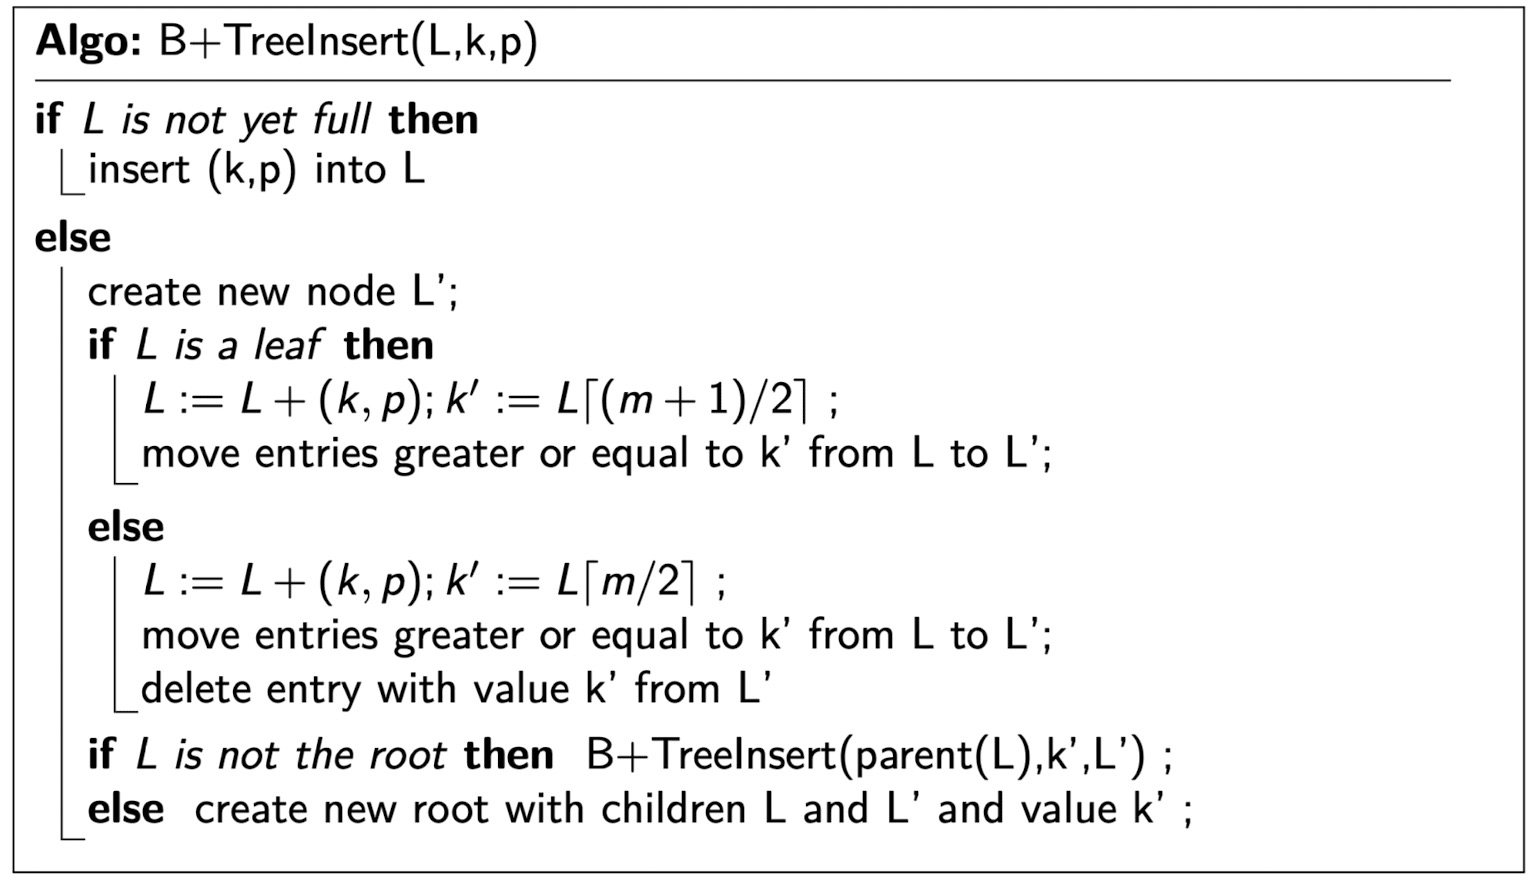
\includegraphics[width=1\linewidth]{images/Screenshot 2024-05-22 at 16.58.30.jpg}
  \caption{Insertion}
  \label{fig:test1}
\end{minipage}%
\begin{minipage}{.5\textwidth}
  \centering
  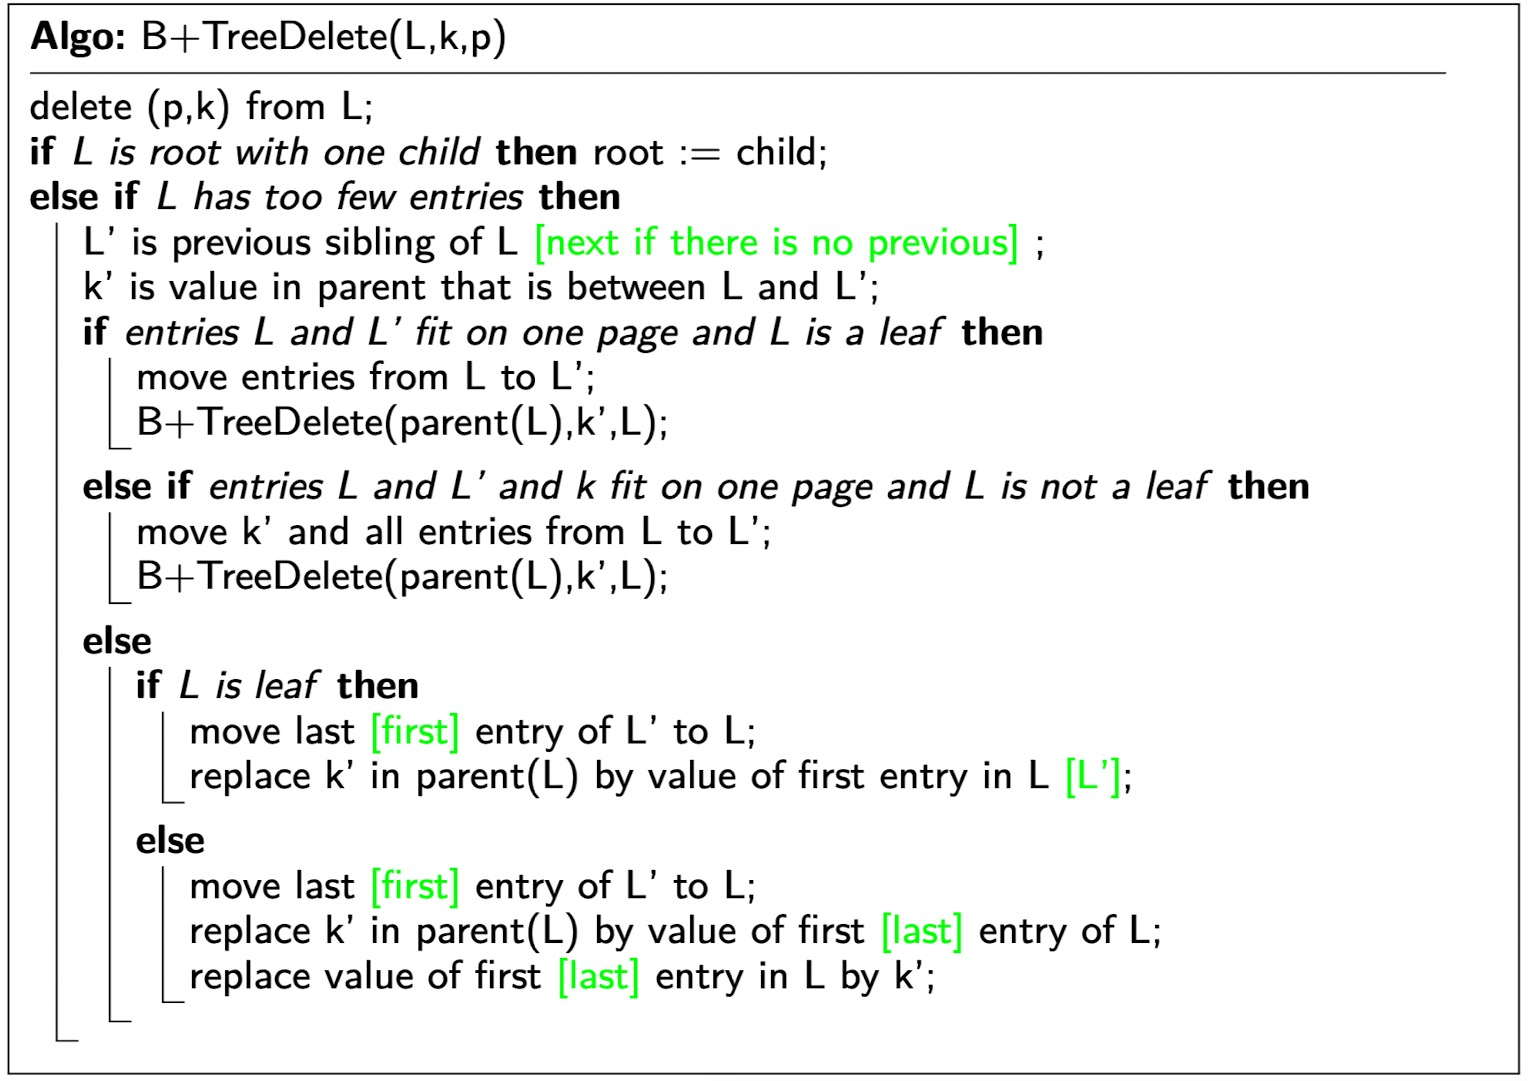
\includegraphics[width=1\linewidth]{images/Screenshot 2024-05-22 at 16.59.12.jpg}
  \caption{Deletion}
  \label{fig:test2}
\end{minipage}
\end{figure}



\subsubsection{Hashing}
\begin{itemize}[label=\(\rhd\)]
    \item Disadvantage of sequential and B+ tree index file organization
    \begin{itemize}[label=\(\rhd\)]
        \item B+ tree: index structure must be accessed to locate data (good for very few lookups, but not good for many lookups as in joins)
        \item Sequential file: binary search on large file might be required
        \item This leads to additional block IO
    \end{itemize}
    \item \textbf{Hashing}
    \begin{itemize}[label=\(\rhd\)]
        \item Provides a way to avoid index structures and to access data directly 
        \item Provides also a way of constructing indexes
    \end{itemize}
    A \textbf{bucket} is a unit of storage containing one or more records
    \item \textbf{Hash file organization}
    \begin{itemize}[label=\(\rhd\)]
        \item We obtain the bucket where a record is stored directly from its search key value using a hash function
        \begin{itemize}[label=\(\rhd\)]
            \item Constant access time
            \item Avoids the use of an index
        \end{itemize}
        \item \textbf{Hash function h}: A function from the set of all search key values $K$ to the set of all bucket addresses $B$
        \begin{itemize}[label=\(\rhd\)]
            \item Worst hash function maps all search key values to the same bucket
            \item An \textbf{ideal hash function} has the following properties:
\begin{itemize}[label=\(\rhd\)]
    \item The distribution is uniform, i.e., each bucket is assigned the same number of search key values from the set of all possible values
    \item The distribution is random, so in the average case each bucket will have the same number of records assigned to it irrespective of the actual distribution of search key values in the file 
\end{itemize}
    \item A \textbf{typical has function}: Perform computation on the internal binary representation of the search key
        \end{itemize}
        \item Records with different search key values may map to the same bucket; thus entire bucket has to be searched sequentially to locate a record
    \end{itemize}
    \item \textbf{Bucket overflow}: If a bucket has not enough space, two reasons:
    \begin{enumerate}
        \item \textbf{Insufficient buckets}: the number of buckets $n_B$ must be chosen to be $n_B> n/f$, where $n=$ total number of records and $f=$ number of records in bucket
        \item \textbf{Skew in distribution of records}
    \end{enumerate}
    \begin{itemize}[label=\(\rhd\)]
        \item \textbf{Overflow chaining (closed hashing)}
        \begin{itemize}[label=\(\rhd\)]
            \item If a record is inserted into bucket $b$, and $b$ is already full, an \textbf{overflow bucket} is provided, where the record is inserted (chained together in a list)
        \end{itemize}
    \end{itemize}
    \item \textbf{Hash Index}: Organizes the search key values with their associated record pointers into a hash file structure
    \begin{itemize}[label=\(\rhd\)]
        \item Buckets contain search keys and pointer to the data records
        \item Multiple (search key, pointer)-pairs might be required
    \item Fixed set $B$ of bucket addresses presents a serious problem (as DBs grow and shrink over time)
    \end{itemize}
    \item \textbf{Dynamic hashing}: Allows the hash function to be modified dynamically
    \item \textbf{Extendable hashing}: one form of dynamic hashing 
    \begin{itemize}[label=\(\rhd\)]
        \item General structure:
        \begin{itemize}[label=\(\rhd\)]
            \item $i$ indicates the number of bits that are used from the hash value
            \item Consecutive entries may point to the same bucket (leads to a smaller prefix associated with this bucket)
        \end{itemize}
        \item \textbf{Lookup}: Locate the bucket containing search key value $K_j$
        \begin{enumerate}
            \item Compute $h(K_j)=X$
            \item Use the first $i$ (hash prefix) high order bits of $X$ as a displacement into the bucket address table, and follow the pointer to the appropriate bucket
        \end{enumerate}
        \item \textbf{Insertion} of a record with search key value $K_j$
        \begin{enumerate}
            \item Use lookup to locate the bucket, say bucket $j$
            \item \textbf{If} there is room in bucket $j$ \textbf{then}
            \begin{itemize}[label=\(\rhd\)]
                \item[] Insert record in bucket
            \end{itemize}
            \item \textbf{Else}: The bucket must be split and insertion re-attempted
            \begin{itemize}[label=\(\rhd\)]

                    \item \textbf{If} $i> i_j$ (more than one pointer to bucket $j$) \textbf{then} 
                    \begin{itemize}[label=\(\rhd\)]
                        \item Allocate new bucket $z$ and set $i_j$ and $i_z$ to old $i_j+1$ 
                        \item Update bucket address table entries that point to $j$ according to prefix
                        \item Remove and reinsert each record in bucket $j$
                        \item Recompute new bucket for $K_j$ and insert record in the bucket
                    \end{itemize}
                    \item \textbf{If} $i=i_j$ (only one pointer to bucket $j$) \textbf{then}
                    \begin{itemize}[label=\(\rhd\)]
                        \item Increment $i$ and double the size of the bucket address table
                        \item Replace each entry in the table by two entries that point to the same bucket
                        \item Recompute new bucket address table entry for $K_j$

                \end{itemize}
            \end{itemize}
        \end{enumerate}
        \item \textbf{Deletion} of a key value $K$
        \begin{enumerate}
            \item Locate $K$ in its bucket and remove it (search key from bucket and record from the file)
            \item The bucket itself can be removed if it becomes empty (with appropriate updates to the bucket address table)
            \item Coalescing of buckets can be done (can coalesce only with a buddy bucket having same value of $i_j$ and same $i_j-1$ prefix, if it is present)
            \item Decreasing bucket address table size is also possible
        \end{enumerate}
        \item \textbf{Benefits} of extendable hashing
        \begin{itemize}[label=\(\rhd\)]
            \item Hash performance does not degrade with growth of file
            \item Minimal space overhead
            \item No buckets are reserved for future growth, but are allocated dynamically
        \end{itemize}
        \item \textbf{Disadvantages}
        \begin{itemize}[label=\(\rhd\)]
            \item Extra level of indirection to find desired record
            \item Bucket address table may itself become very big
            \item Changing size of bucket address table is expensive
        \end{itemize}
    \end{itemize}
\end{itemize}

\subsubsection{Index Definition in SQL}
\begin{itemize}[label=\(\rhd\)]
    \item Create an index:
    \begin{itemize}[label=\(\rhd\)]
        \item[] \textbf{create index} <IdxName> \textbf{on} <RelName> (<AttrList>)
    \end{itemize}
    \item Drop an index:
    \begin{itemize}[label=\(\rhd\)]
        \item[] \textbf{drop index} <index-name>
    \end{itemize}
\end{itemize}



